\documentclass[iop,apj]{emulateapj}
\usepackage{amsmath,amssymb,amstext}
\usepackage{todonotes}
\usepackage[breaklinks,colorlinks,citecolor=blue,linkcolor=magenta]{hyperref} 
\renewcommand*{\sectionautorefname}{Section}
\usepackage[all]{hypcap} %Links go to figures; breaks on deluxetables (use \capstartfalse \capstarttrue to fix it)

\usepackage{aas_macros}
\usepackage{natbib}
\bibliographystyle{apj}

\shorttitle{Short Title}
\shortauthors{Author et al.}

\begin{document}

\title{Detecting Active Asteroids/Comets from OSSOS survey images}
\author{Authors}
\affil{Affiliations}

\begin{abstract}
Abstract.
\end{abstract}

\keywords{keywords}
\maketitle

\section{Introduction}
% so far, im not making a point of using good wording
% definietly have to go back and add in citations

The active asteroids are small bodies in the main asteroid belt which have transient dust emission producing comet-like comae and tails. Unlike comets, which originate in the Kuiper Belt and Oort cloud and have been scattered inwards by gravitational effects, the active asteroids have  stable orbits confined to the main belt and likely formed in the same location as they reside presently \citep{sheppard14}. For objects which formed in the the outer region of the main belt, beyond the snow line, the crystallized water ice which was present at the time of formation and not exposed to primordial heating may still remain in reservoirs beneath the surface \citep{sonnett11}.  According to models done by \citet*{fanale89},  beyond heliocentric distances of 2.4 AU ice can be protected against sublimation by a 'relatively thin' surface regolith  of depth 1 -- 100 m for the entire age of the solar system. If the ice layer were to be exposed to sub solar heating,  sublimation could be triggered,  ejecting dust particles from the surface producing a coma.  %Objects in the main asteroid belt which are driven by sublimation are also named Main Belt Comets (MBCs). 
The source of the dust emission may be different for each object and could include ice sublimation, impact ejecta, rotational instabilities due to YORP torques, or a combination of several effects. \citep{hsieh15}. %; these objects are known as disrupted asteroids. 
As the source of the observed activity may not be a result of cometary ice sublimation, these objects are better known as active asteroids. Main belt comets are a subset of this group where ice sublimation is thought to be the source of the dust emission. 

% As the presence of ice in the inner solar system could be important for determining the chemistry of the early solar nebula and planet formation, it is worth while to determine what the source of the activity is. 
% impacts inferred from observed large brightening and quick fading 
% sublimation inferred from prolonged or periodic activity during perihelion passage, Hsieh et al 2010, 2011

%The ejected dust would form a coma around the object, and radiation pressure affects would then (preferentially) push the smaller particles away from the asteroid forming a tail.

%Sublimation driven active asteroids differ from comets in that the comets, having larger ice reservoirs, would have stronger sublimation events which could eject larger debris. The cometary tail would then be longer lived as the larger debris would be less effected by the radiation pressure, and thus dissipate slowly. It is also possible, however, that prolonged activity is a result of ongoing ejection of small, fast dissipating particles. \cite{TEST} 

Since the first discovery of an active main-belt asteroid, 133P/Elst-Pizarro, several attempts have been made to identify new objects of this type; at present, eighteen objects have been identified (refer to Figure 1) \citep{jewitt15}. A comprehensive review of such searches can be found in \citet{hsieh15}.  A persistent challenge to this effort is that the detection of the coma or tails around small dark objects is highly dependent on the magnitude constraints of the survey. As most asteroids fall near the limiting magnitude of the survey in which they are discovered \citep{jewitt15}%(is this cite necessary?)
, objects which are larger, closer, or have higher albedo are preferentially detected and any dust emission would be more easily apparent. The active fraction of identified active asteroids greater than 1 km to main belt asteroids greater than 1 km is $f \, \sim \, 10^5$, and describes a strong lower limit as many objects are yet undetected. \citep{jewitt15} %From a study of 30,000 objects observed near perihelion, \cite{} Hsieh et all (2015) concluded that $f \, \sim \, 10^4$ for asteroids which are active at any instant in the outer belt.


% WHAT IS NEW, BETTER, DIFFERENT ABOUT OSSOS???
Previously undetectable emission activity may be able to be identified from the Outer Solar System Origins Survey (OSSOS) which was designed to detect trans neptunian objects, and has a low limiting magnitude of 24.5 mag. The survey covers a wide field of both the ecliptic plane and low inclinations, and observes with long ($>$ 287 s) exposures, allowing for the potential serendipitous discovery of active dust emission which was previously too faint to detect. In this study we intend to observe numbered asteroids in the OSSOS data set and identify potential activity by measuring the point spread function (PSF).

% area search is attempted to be few stars

\section{Observations}

Observations taken by OSSOS with the Canada-France-Hawaii telescope (CFHT) MegaPrime wide-field optical imaging facility  at the summit of Mauna Kea, Hawaii, have been collected since 2013. The wide-field imager, MegaCam, consists of a 36 CCD image plane, each 2048 x 4125 CCD with resolution of 0.185"/pix. This covers a field of  roughly 1$^{\circ}$ x 1$^{\circ}$ on the sky. Each block of data taken consists of a mosaic of 21 segments of one-square-degree sky coverage, and at present, covers two orbital phase spaces on the plane of the ecliptic, and two off plane at low inclinations. MegaCam observes in the optical to near infrared with filters u*, g', r', i', and z'. Of these, r' and u* are the best suited filters for observing main belt objects, and the analysis presented only includes observations made using these filters. \todo{reword!}

% how is the image data calibrated? filters, S/N? MOPS?
The OSSOS images are reduced ... \todo{how reduced}. (standard data detrending???) Source characteristic measurements were obtained from source extraction \todo{citep(sep)} and were used to extract the orbital information the transient object. 


%As the identified active asteroids do not share a specific phase space the analysis was not constrained to just the main belt or plane of the ecliptic, but for all known objects with heliocentric distances beyond the inner belt (a \textgreater \, 2.064 AU), inclinations below 40$^{\circ}$, and eccentricity less than 0.45. 
% to detect objects in the main asteroid belt, objects with semimajor axis 2.064 < a < 3.277 AU, e < 0.45, i < 40 deg
% PSF detections
% cuts, identifying process

\section{Analysis}

\todo{rewrite with proper good english}
We analyze as set of 3528 images with exposure times greater than 200s, with (\todo{fill in}) observations of (\todo{fill in}) established main-belt objects from the OSSOS survey. This study exclusively worked with known objects as they could easily be identified in each exposure from the asteroids predicted arc and observables. Additionally, from the coordinates that we calculate the asteroid to be at, we can refine the objects arc. 

An automated pipeline was written to identify each asteroid in an OSSOS exposure by, in order of 'priority': it's location relative to the predicted coordinates,  elongation due to trailing effects, and apparent magnitude. The elongation condition was calculated from the predicted motion of the asteroid over the length of the exposure, and approximated as an ellipse which could be compared to the shape parameters calculated by the photometry. Asteroids which were not the expected shape, but satisfied the coordinate and magnitude condition were flagged for human inspection. Cases of the asteroid being too close to bad pixels, the edge of the CCD, or involved with bright sources would be removed at this step of the pipeline. For exposures where the elongation ratio was greater than 1:5 ***** the photometry measured the asteroid as two separate sources, and the image was flagged for human inspection. If more than one source met the same level of criteria but the object was not expected to be greatly elongated, the image was flagged separately for review.

In order to accurately measure the PSF of the asteroid, which is necessary to check for anomalous flux surrounding the object that could indicate activity, it is necessary to ensure that the asteroid is isolated from other sources. From a comparison with a catalogue of bright sources built for the OSSOS images \citep{ossos}, the cases where the asteroid was involved could be discarded.

To ensure that no asteroid could not be accounted for in the pipeline process, exposures where no source was found by the photometry in the region surrounding the predicted location of the asteroid, no objects met the elongation nor magnitude conditions, and images which failed to be processed by the photometry were also recorded to be reprocessed.

% Additional work was done to compare the observed light curves with the Asteroid Lightcurve Database (LCDB, \citep{warner08})

To calculate the PSF of the asteroid, the image was rotated to align the elongation to the horizontal axis, and for a small segment of 2.5 *** times the full-width-half-maximum (FWHM) the flux was summed for each row. The flux was then plotted as a function of position across the image and fitted to a Gaussian/Moffat function. The same processes was followed for a mean PSF of bright stars in the same exposure built from the OSSOS MOP pipeline \citep{ossos}. The fitted functions were then compared to check for a greater than 2 sigma **** deviation in the wings of the PSF. Due to saturation effects along the core of the asteroid, and the requirement of the rotation of the image before reading out the flux, asteroids with a lower magnitude than 18.5 mag were excluded as the PSF could not be accurately calculated. 



\section{Discussion}

As the involvement check was preformed using a catalogue of bright objects, it is possible that some asteroids identified and carried through the pipeline process were involved with dim background objects. An example of this is shown in figure 3. Depending on the geometry of the involvement this could be selected as an asteroid with activity, possibly a large bright jet. In order to distinguish between activity and involvement, the asteroids with unusual PSF's were all manually reviewed. Through this process we could determine whether a jet was present, in which case the outflowing dust would also have a trailing effect through the exposure, or if it were a case of involvement. We do not expect that a jet would be present for a fraction of the exposure time during one observation. 


\acknowledgments{
  Acknowledgments. 
}

\bibliographystyle{plainnat}
\bibliography{mbc_paper}

% to be updated when the new get_iamges for all objects in families has been completed
\begin{figure}[!htb]
    \centering
    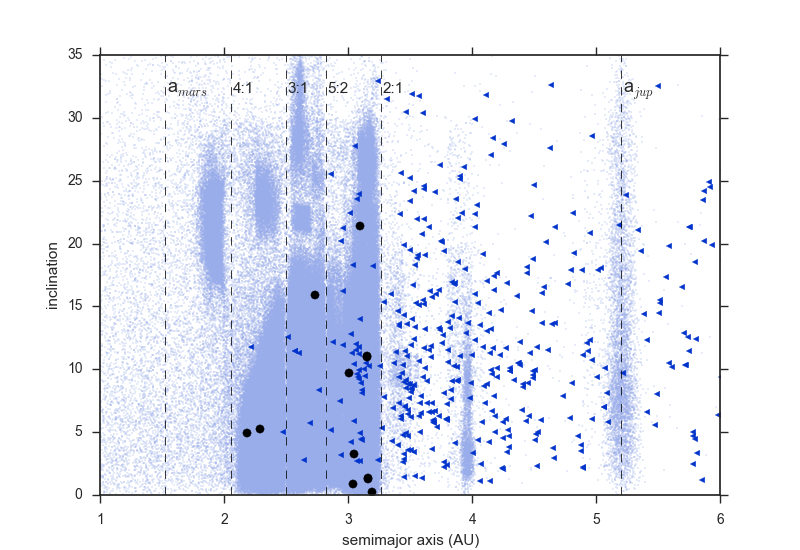
\includegraphics[height=9cm]{graphs/aa_comets_mba_all.png}
    \caption{Inclination of all known objects in the main asteroid belt as a function of semimajor axis.  Mean motion resonances between Mars and Jupiter as well as the planet's semimajor axis are marked in dashed lines, main belt objects are marked as light small dots, comets as arrows, and active asteroids as stars. \cite{mpc}}\label{fig:1}
\end{figure}

\begin{figure}[!htb]
    \centering
    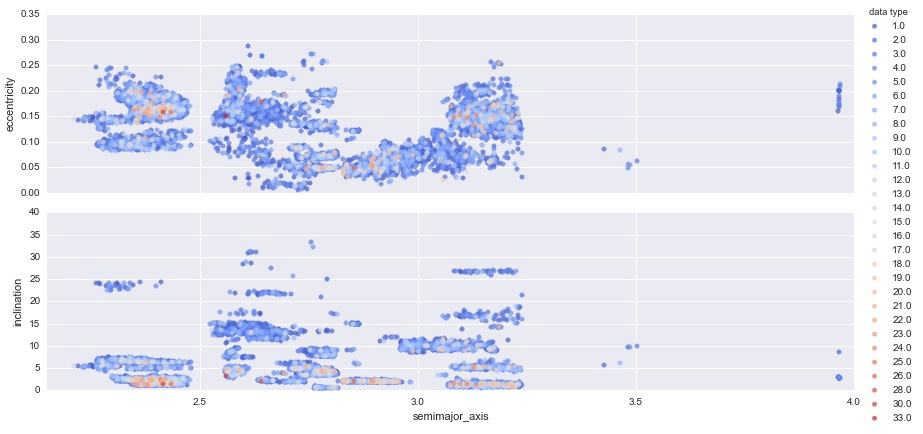
\includegraphics[height=7cm]{graphs/a_e_i_occur.png}
    \caption{Inclination and eccentricity as a function of semi-major axis of all objects. Colours represents number of observations (occurrences) used in the analysis}\label{fig:2}
\end{figure}

\begin{figure}[!htb]
    \centering
    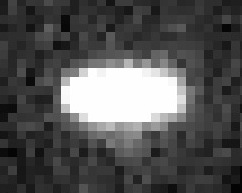
\includegraphics[height=4cm]{images/background_gal.jpeg}
    \caption{An asteroid involved with a dim background object. }\label{fig:3}
\end{figure}


\end{document}



